\subsection{Profiling}


\begin{frame}
  \begin{block}{Introduction to \textbf{pbdPROF}}
    \begin{itemize}
      \item Successful Google Summer of Code 2013 project.
      \item Available on the CRAN.
      \item Enables profiling of MPI-using R scripts.
      \item \pbdR\ packages officially supported; can work with others\dots
      \item Also reads, parses, and plots profiler outputs.
    \end{itemize}
  \end{block}
\end{frame}


\begin{frame}
  \begin{block}{How it works}
  MPI calls get hijacked by profiler and logged:
	\begin{center}
	  \ \hspace{2cm}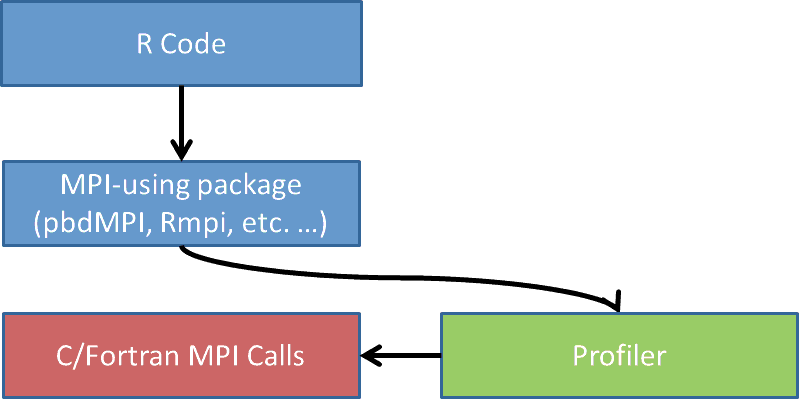
\includegraphics[width=0.8\textwidth]{../common/pics/prof/mpi_profiler}
	\end{center}
  \end{block}
\end{frame}


\begin{frame}
  \begin{block}{Introduction to \textbf{pbdPROF}}
    \begin{itemize}
      \item Currently supports the profilers \textbf{fpmpi} and \textbf{mpiP}.
      \item \textbf{fpmpi} is distributed with \textbf{pbdPROF} and installs easily, but offers 
minimal profiling capabilities.
      \item \textbf{mpiP} is fully supported also, but harder to install.
    \end{itemize}
  \end{block}
\end{frame}



\subsection{Installing pbdPROF}

\begin{frame}
  \begin{block}{Installing \textbf{pbdPROF}}
    \begin{enumerate}
      \item Build \textbf{pbdPROF}.
      \item Rebuild \textbf{pbdMPI} (linking with \textbf{pbdPROF}).
	  \item Run your analysis as usual.
	  \item Interactively analyze profiler outputs with \textbf{pbdPROF}.
    \end{enumerate}
  \end{block}
\end{frame}


\begin{frame}[fragile]
  \begin{block}{Build \textbf{pbdPROF}}
\begin{lstlisting}[language=shl,title=\ ]
R CMD INSTALL pbdPROF_0.2-1.tar.gz
\end{lstlisting}
    \begin{itemize}
      \item The above installs \textbf{fpmpi}.
      \item \textbf{mpiP} can be used if you have a system installation available.
      \item See package vignette for more details and troubleshooting.
    \end{itemize}
  \end{block}
\end{frame}



\begin{frame}[fragile]
  \begin{block}{Rebuild \textbf{pbdMPI}}
\begin{lstlisting}[language=shl,title=\ ]
R CMD INSTALL pbdMPI_0.2-2.tar.gz --configure-args="--enable-pbdPROF"
\end{lstlisting}
    \begin{itemize}
      \item Any package which explicitly links with an MPI library must be rebuilt in this way 
(\textbf{pbdMPI}, \textbf{Rmpi}, \dots).
	  \item Other \pbdR\ packages link with \textbf{pbdMPI}, and so do not need to be rebuilt.
      \item See \textbf{pbdPROF} vignette if something goes wrong.
    \end{itemize}
  \end{block}
\end{frame}

